\section{How do you want to be remembered?}
I'd like to be remembered on my birthday and in the slight facial feature or smile on the faces of some of my descendants.
When folks ponder the story of what happened during the decades in which I lived, perhaps someone will reflect on the way I lived.
I made choices daily that scrapped, marked and sculptured the contours of my life.
Perhaps there will be something of the shape of that life for people to see and understand.

\begin{figure}
\centering
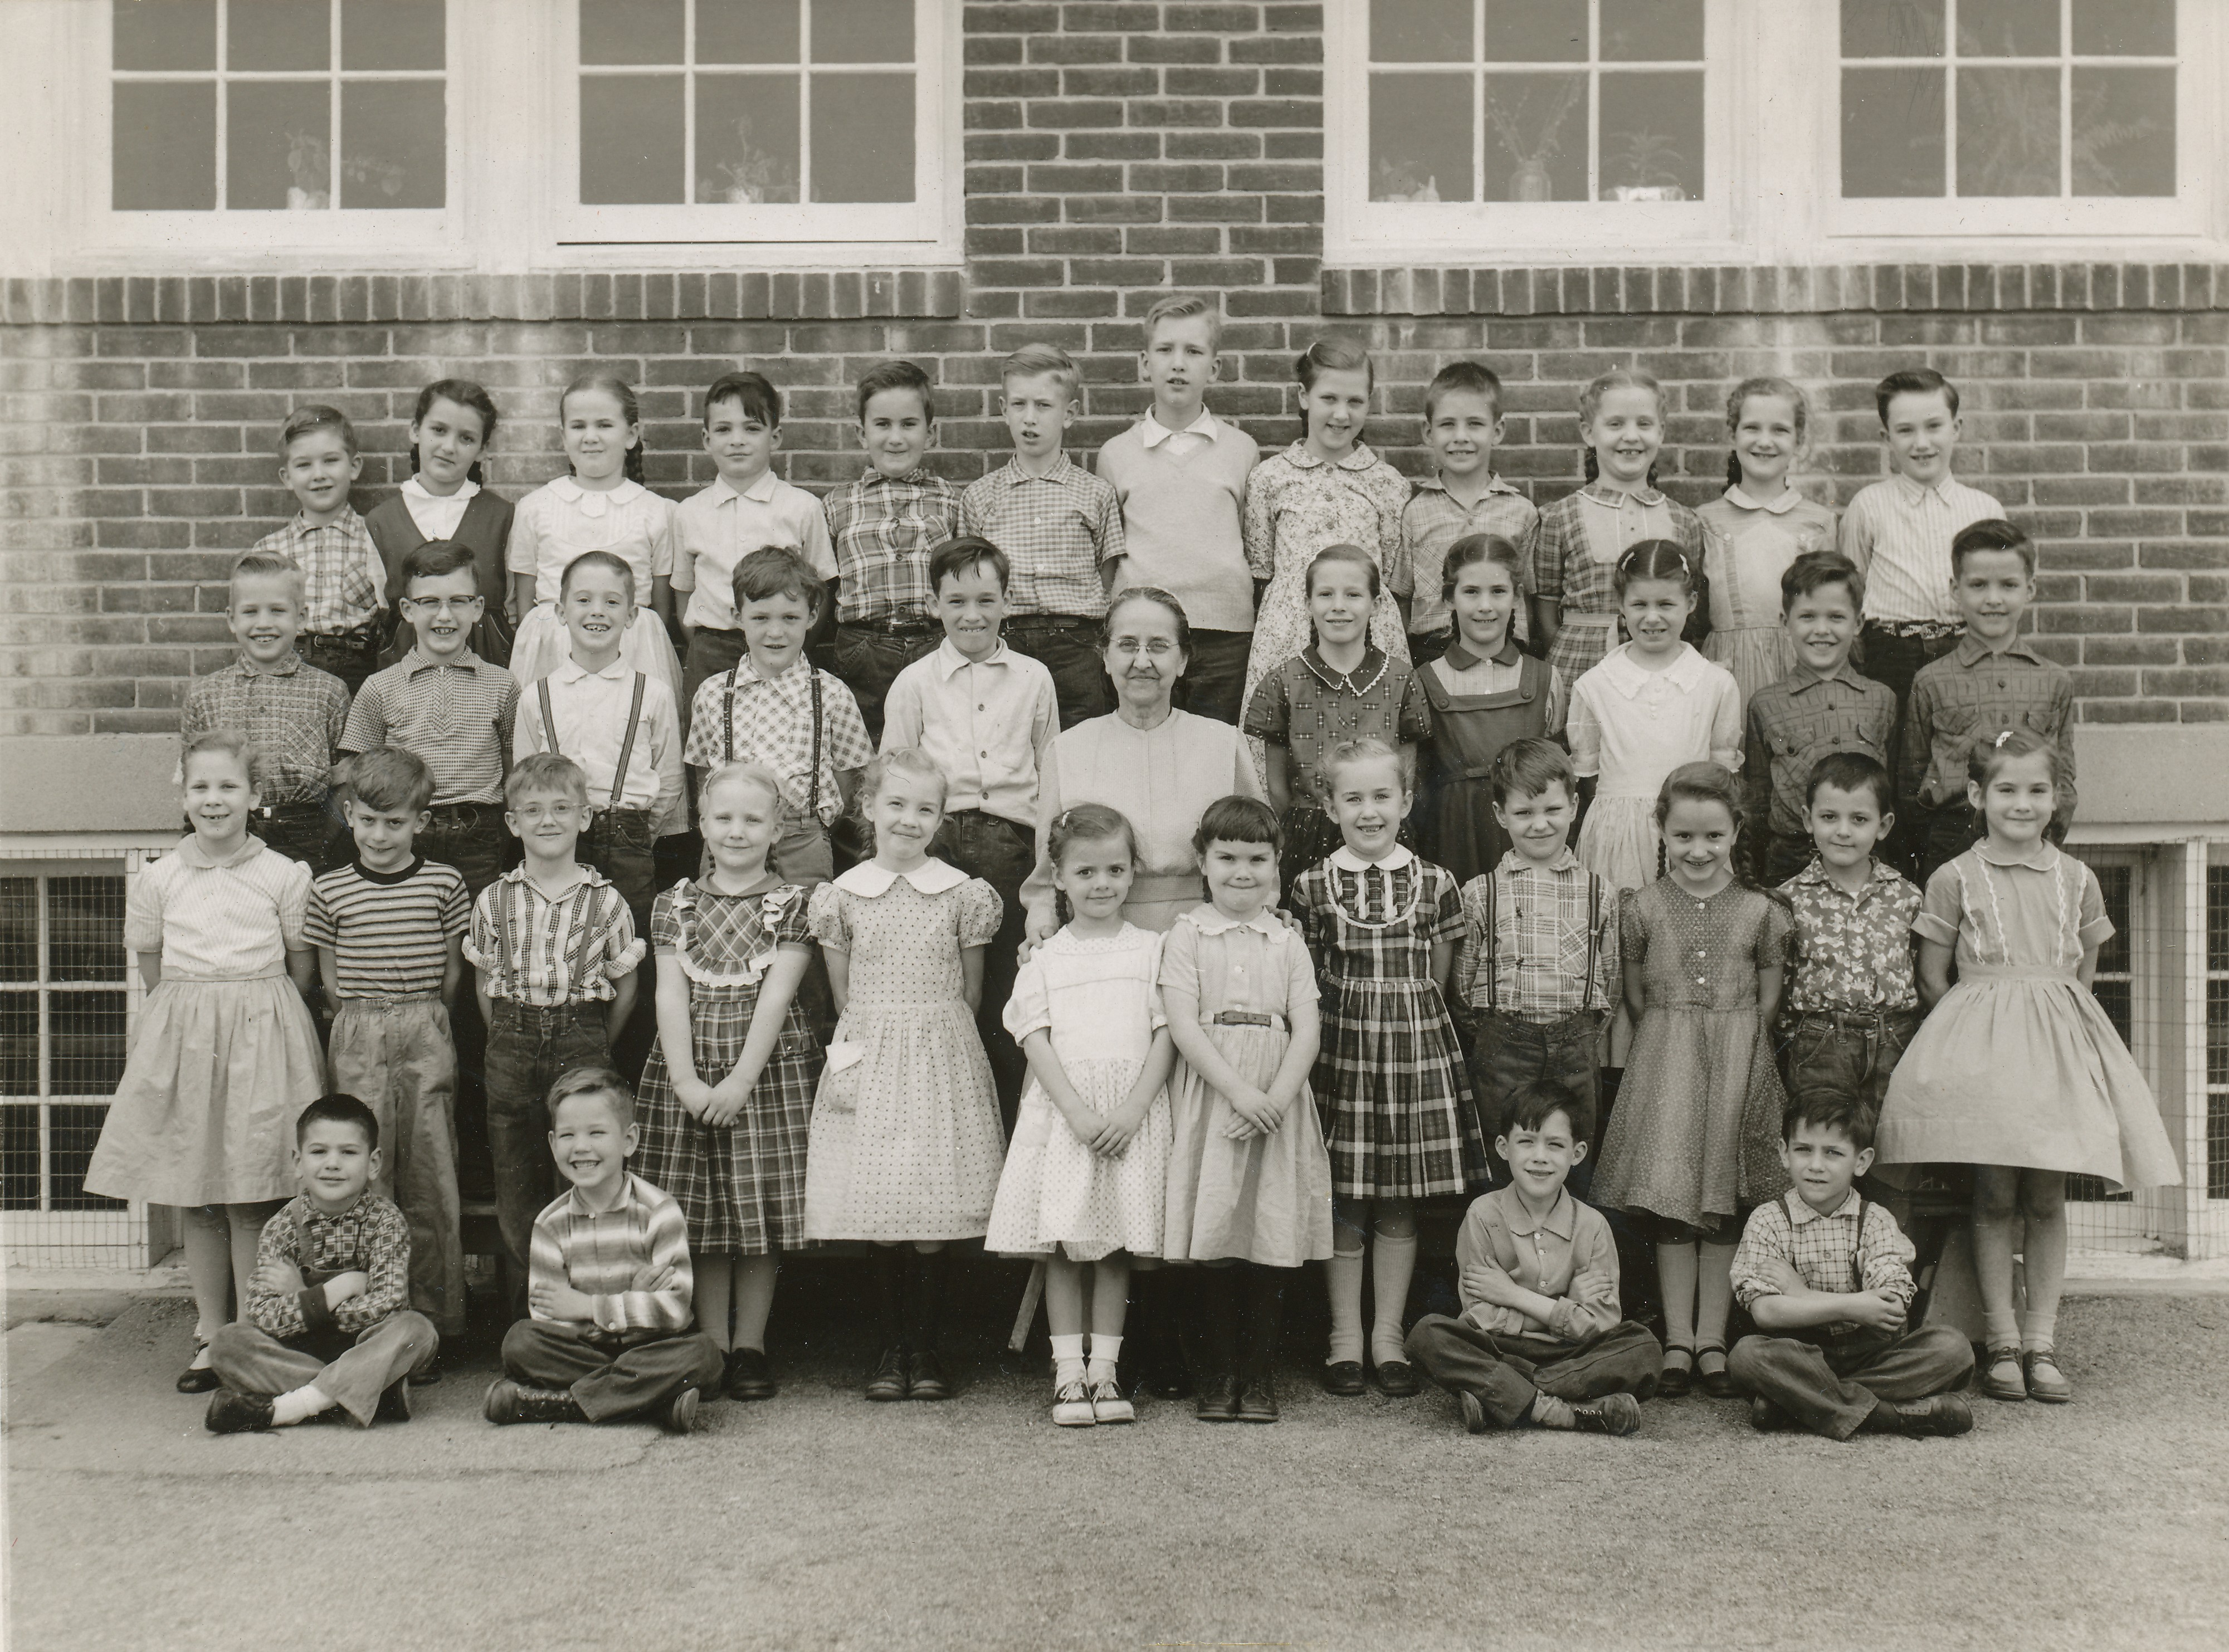
\includegraphics[width=0.9\textwidth]{reflections/14.jpg}
\caption{
Bleeding heart
}
\end{figure}

I hope it is evident that I enjoyed beauty.
The sun rising and setting, the freshness of a lovely northern Indiana June morning, the grandeur of a giant oak tree, the mischief of the squirrels, the amazing detail of a flower, the speed at which the garden grows in a well-watered June, and the rising and setting of the moon.
And so much more as each day has some part to savor.

\begin{figure}
\centering
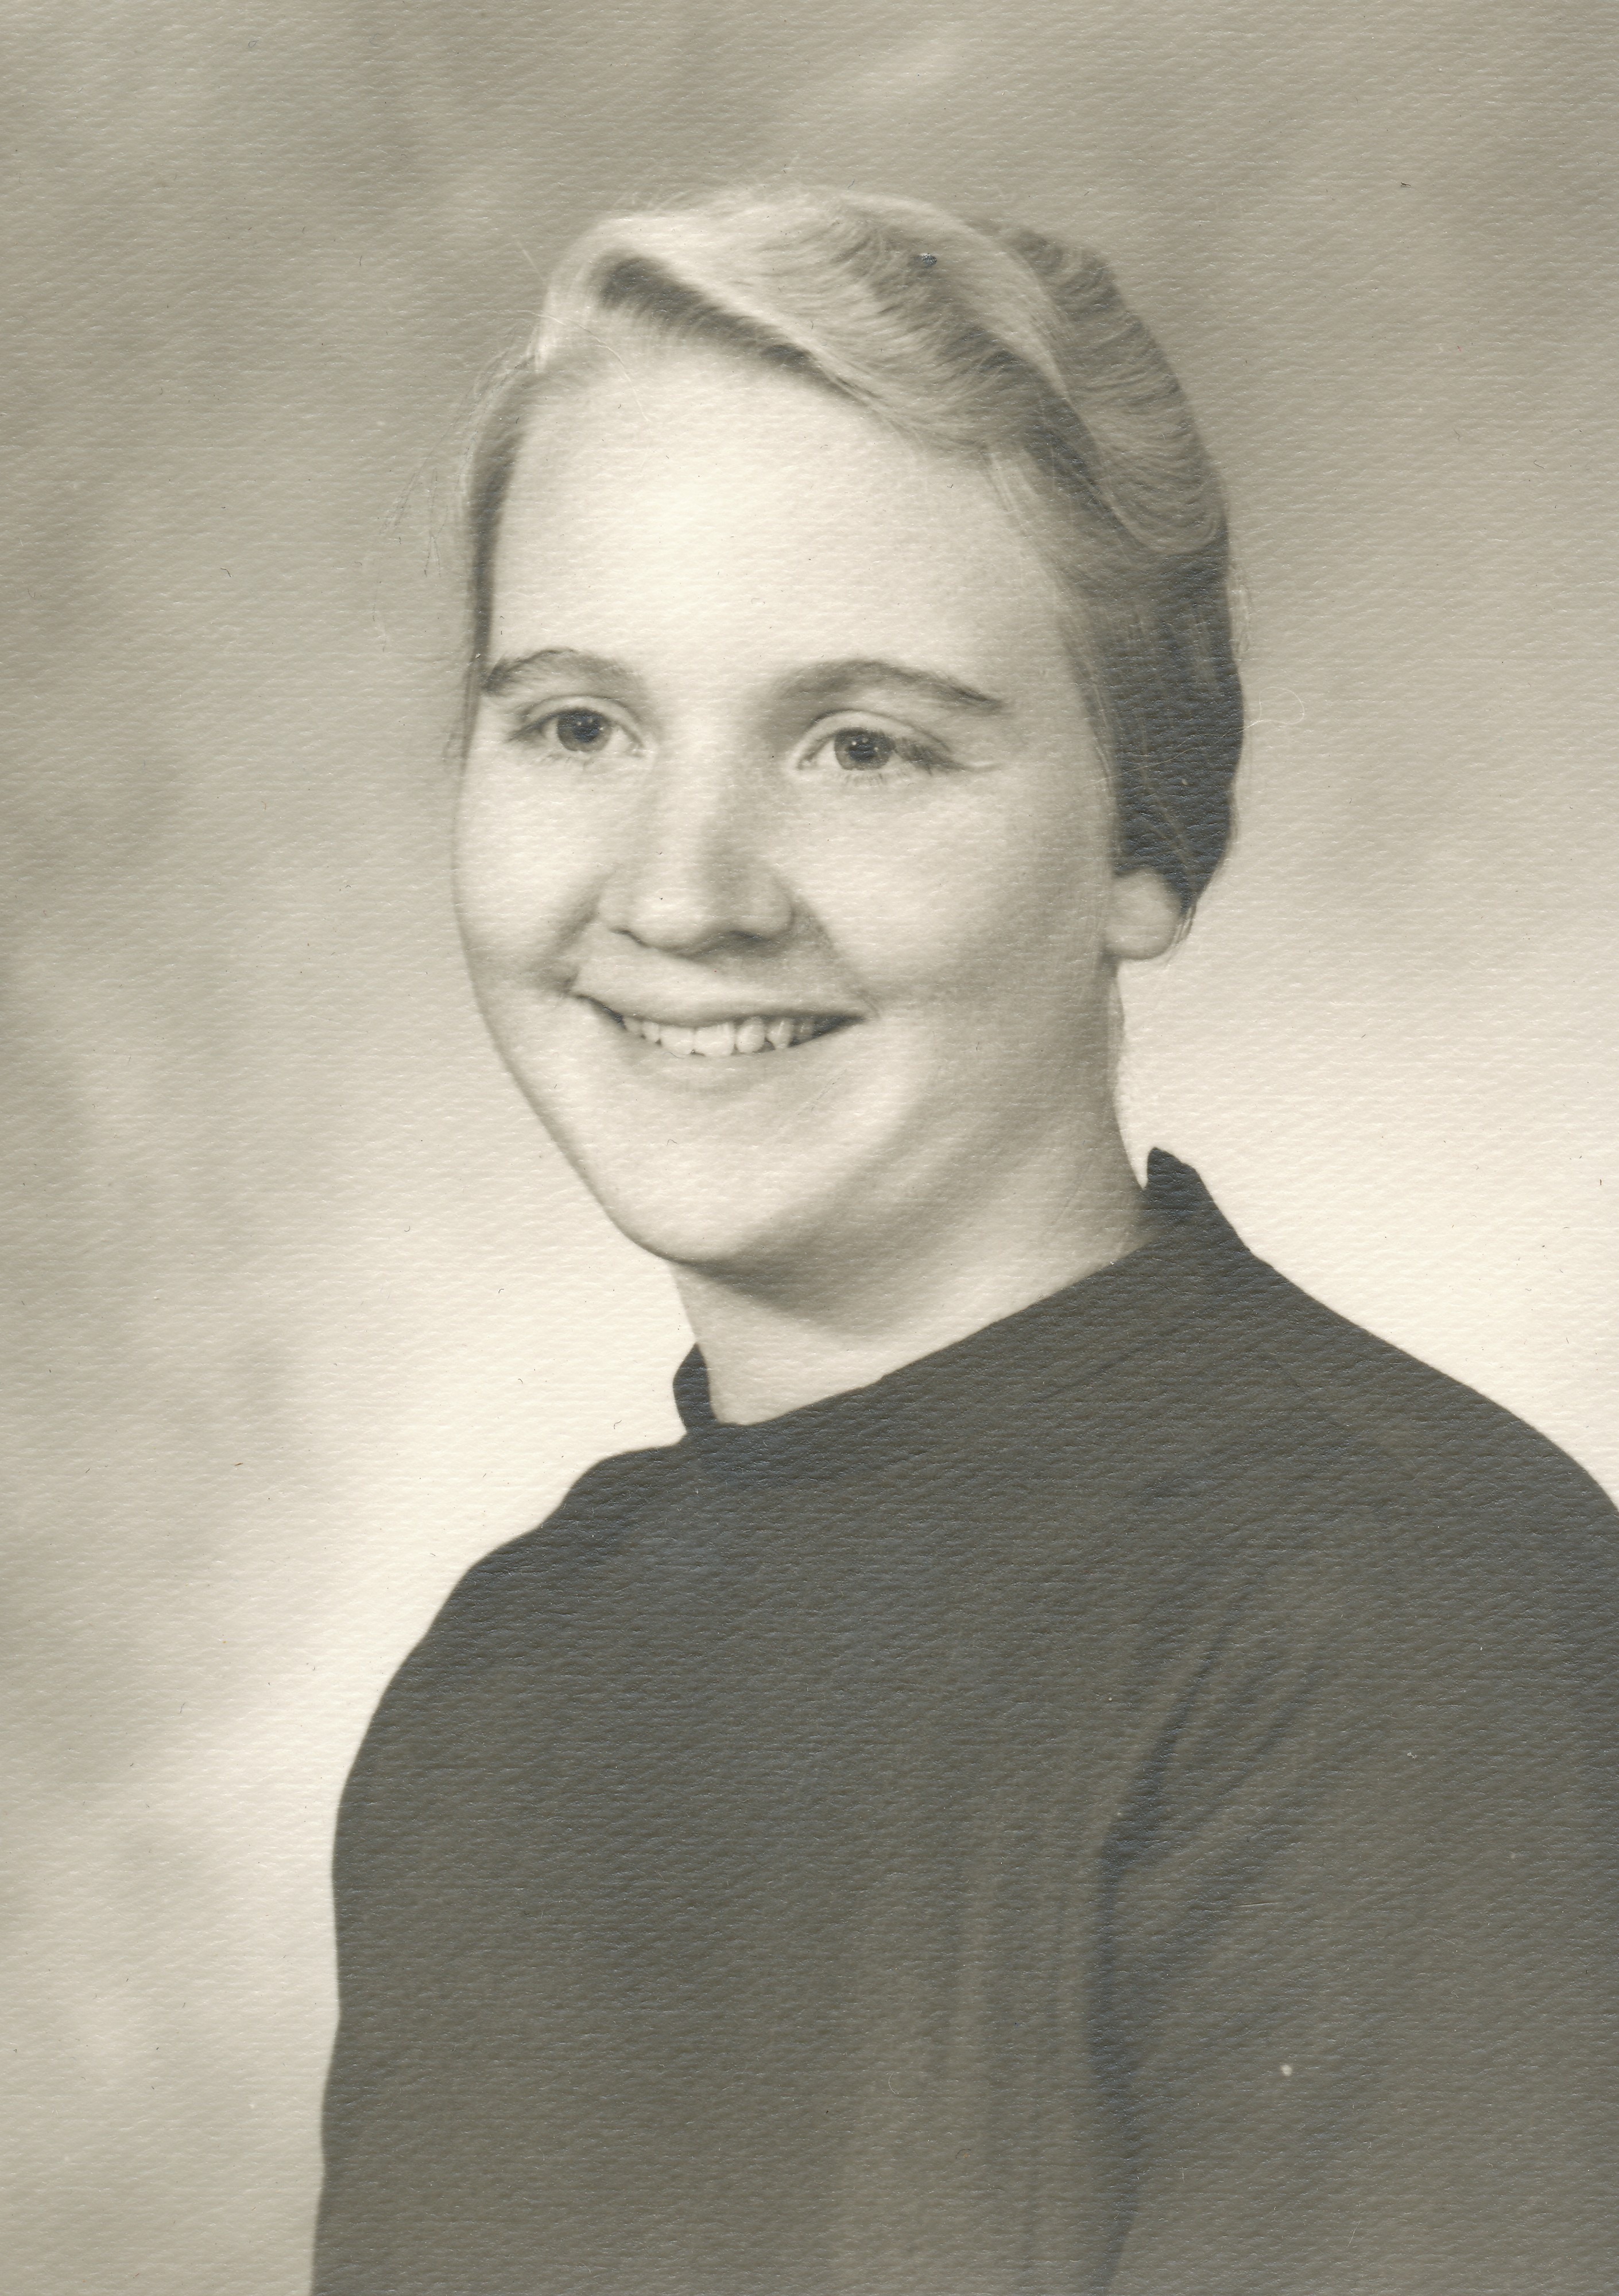
\includegraphics[width=0.9\textwidth]{reflections/15.jpg}
\caption{
Garden at Mayflower Place
}
\end{figure}

I learned that it was not enough to be moved to tears by injustice but that there were actions that could be taken to balance the scales of justice.
When needed I intended to give voice to what needed to be said.
People are so varied and interesting in personality and action.
Listening and hearing another's perspective and meaning added to what I understood about life.
What remains of this effort can perhaps only be seen in the lives of other people being formed alongside mine.
Together we shaped a space we called family and community.
May what is remembered be light for the path ahead.

\begin{figure}
\centering
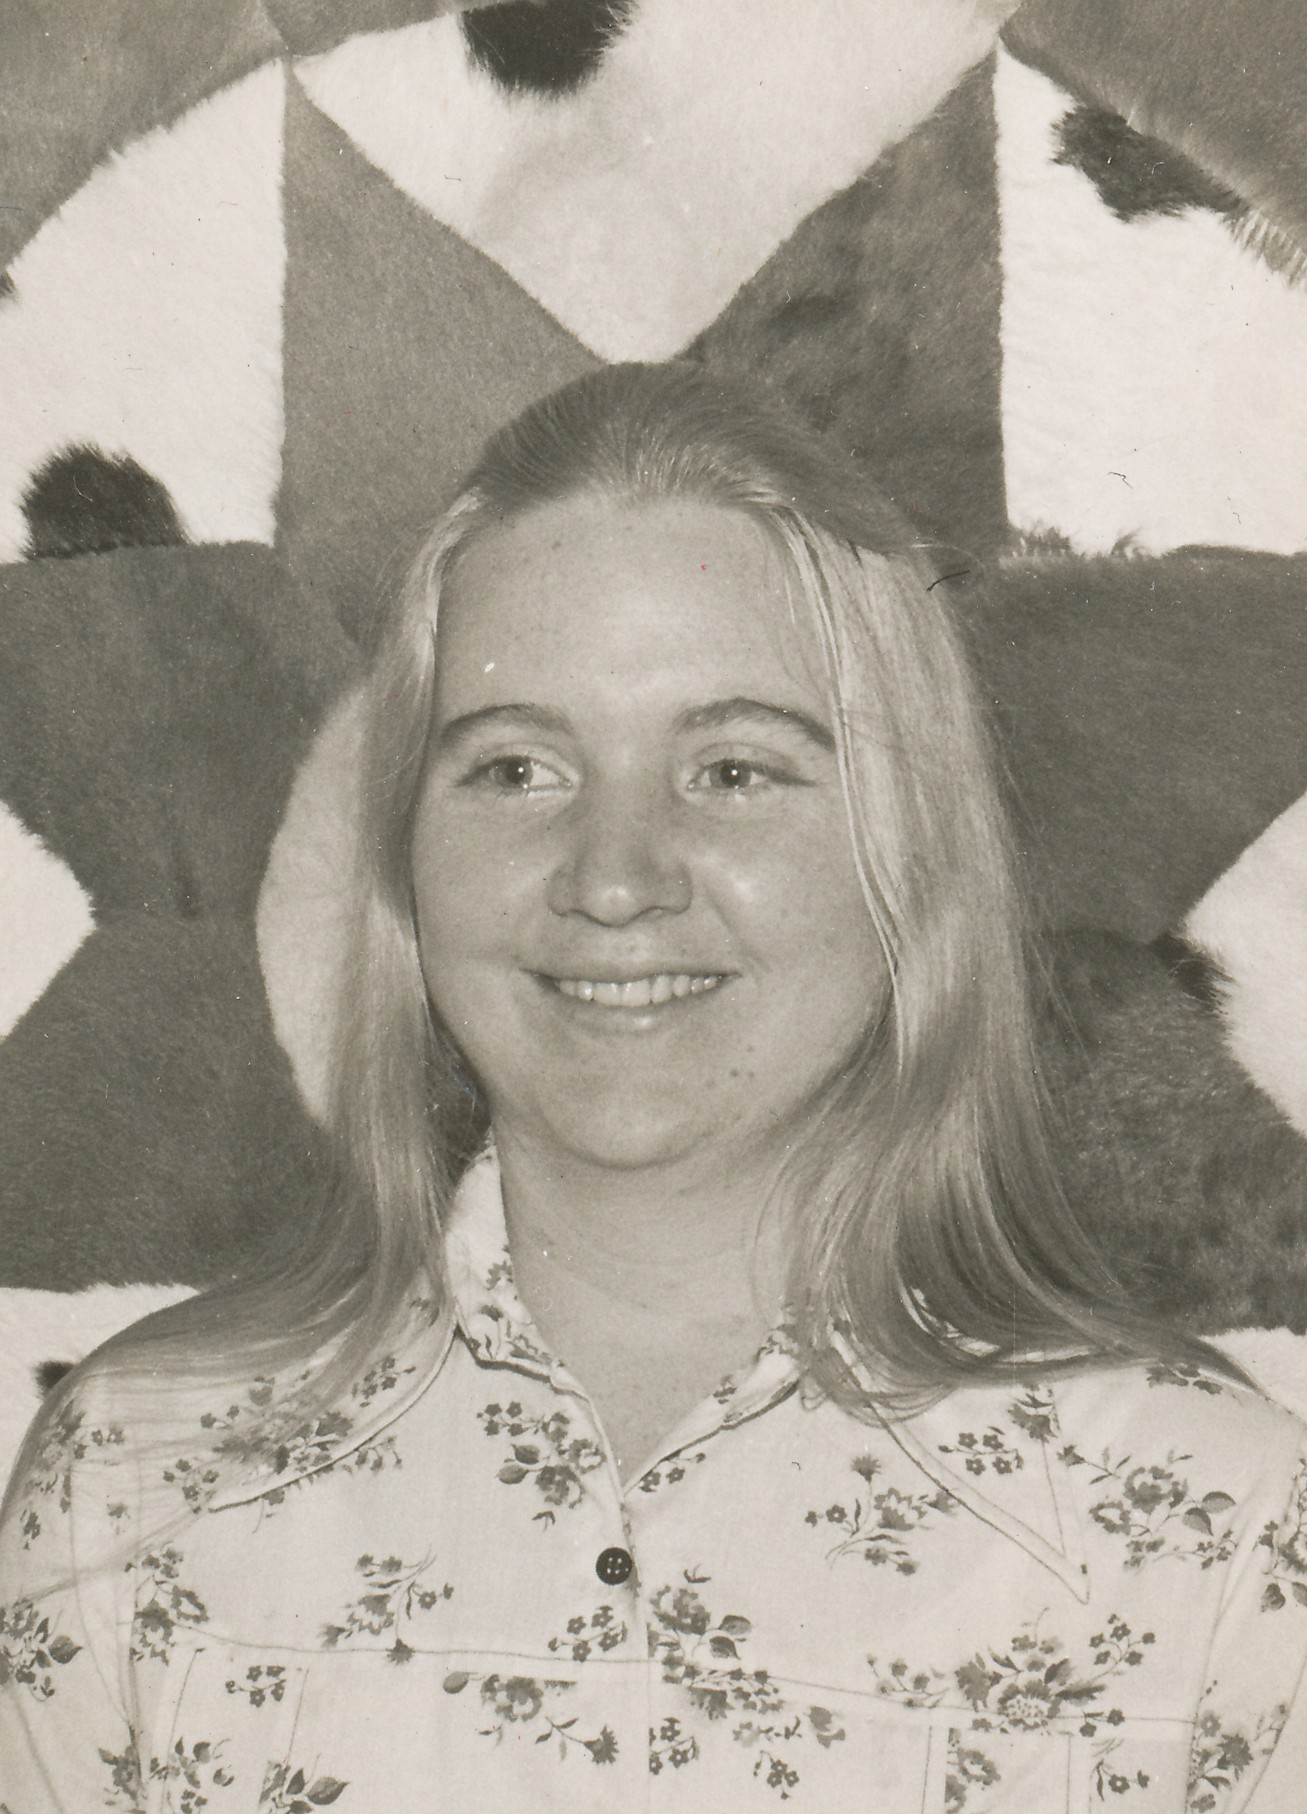
\includegraphics[width=0.9\textwidth]{reflections/17.jpg}
\caption{
Family at the Calendar Garden 2018
}
\end{figure}






